\documentclass[aspectratio=169]{beamer}

\usetheme{default}
\usecolortheme{dove}

\setbeamertemplate{navigation symbols}{}
\setbeamertemplate{footline}{%
  \hfill{\large\insertframenumber\,/\,\inserttotalframenumber}\hspace{0.8em}\vspace{0.5em}%
}

\definecolor{popblue}{RGB}{52, 101, 164}
\definecolor{sampred}{RGB}{204, 0, 0}
\definecolor{paramgreen}{RGB}{0, 140, 70}
\definecolor{warnred}{RGB}{180, 40, 40}
\definecolor{orange1}{RGB}{220, 120, 0}
\definecolor{violet1}{RGB}{120, 50, 160}
\definecolor{lightbg}{RGB}{245, 245, 250}

\setbeamercolor{frametitle}{fg=popblue}
\setbeamercolor{title}{fg=popblue}

\usepackage{pgfplots}
\usepackage{tikz}
\usetikzlibrary{shapes, arrows.meta, positioning, calc, decorations.pathreplacing, patterns}
\pgfplotsset{compat=1.18}
\usepackage{amsmath, amssymb}
\usepackage{pifont}
\usepackage{colortbl}
\usepackage{fontenc}

\title{Statistics: The Complete Picture}
\subtitle{Everything We Learned in 14 Lectures}
\date{}

\begin{document}

% ============================================================
\begin{frame}
\titlepage
\end{frame}

% ============================================================
\begin{frame}
\frametitle{The Journey}

\begin{center}
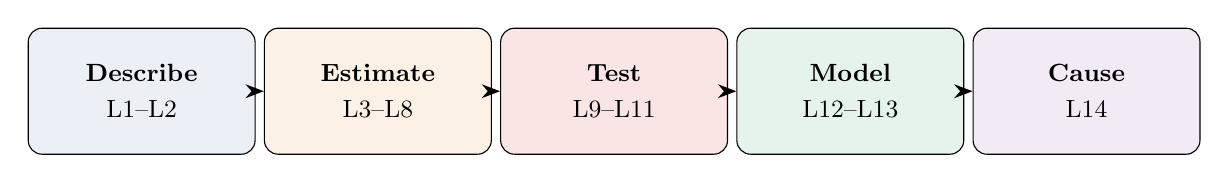
\begin{tikzpicture}[
  phase/.style={draw, rounded corners=5pt, text width=2.6cm, align=center, inner sep=4pt, font=\small, minimum height=1.6cm}
]
  \node[phase, fill=popblue!10] (desc) at (-6, 0) {
    \textbf{Describe}\\[2pt]
    L1--L2
  };
  \node[phase, fill=orange1!10] (est) at (-3, 0) {
    \textbf{Estimate}\\[2pt]
    L3--L8
  };
  \node[phase, fill=sampred!10] (test) at (0, 0) {
    \textbf{Test}\\[2pt]
    L9--L11
  };
  \node[phase, fill=paramgreen!10] (model) at (3, 0) {
    \textbf{Model}\\[2pt]
    L12--L13
  };
  \node[phase, fill=violet1!10] (cause) at (6, 0) {
    \textbf{Cause}\\[2pt]
    L14
  };

  \draw[-{Stealth}, thick] (desc) -- (est);
  \draw[-{Stealth}, thick] (est) -- (test);
  \draw[-{Stealth}, thick] (test) -- (model);
  \draw[-{Stealth}, thick] (model) -- (cause);
\end{tikzpicture}
\end{center}

\vspace{0.3cm}
\begin{center}
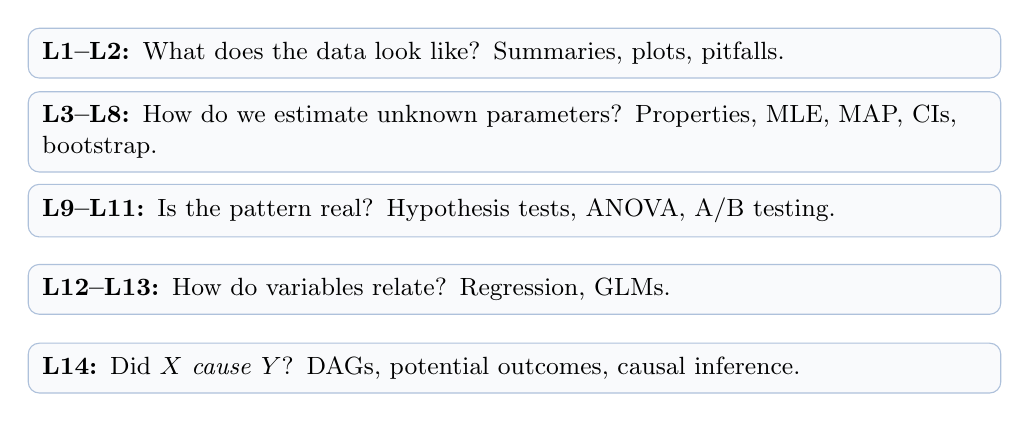
\begin{tikzpicture}[
  sbox/.style={draw=popblue!40, fill=popblue!3, rounded corners=4pt, text width=12cm, align=left, inner sep=5pt, font=\small}
]
  \node[sbox] at (0, 1.5) {\textbf{L1--L2:} What does the data look like? Summaries, plots, pitfalls.};
  \node[sbox] at (0, 0.5) {\textbf{L3--L8:} How do we estimate unknown parameters? Properties, MLE, MAP, CIs, bootstrap.};
  \node[sbox] at (0, -0.5) {\textbf{L9--L11:} Is the pattern real? Hypothesis tests, ANOVA, A/B testing.};
  \node[sbox] at (0, -1.5) {\textbf{L12--L13:} How do variables relate? Regression, GLMs.};
  \node[sbox] at (0, -2.5) {\textbf{L14:} Did $X$ \textit{cause} $Y$? DAGs, potential outcomes, causal inference.};
\end{tikzpicture}
\end{center}
\end{frame}

% ============================================================
% BLOCK 1: FOUNDATIONS & DESCRIPTION
% ============================================================
\begin{frame}
\frametitle{L1--L2: Foundations \& Descriptive Statistics}

\begin{center}
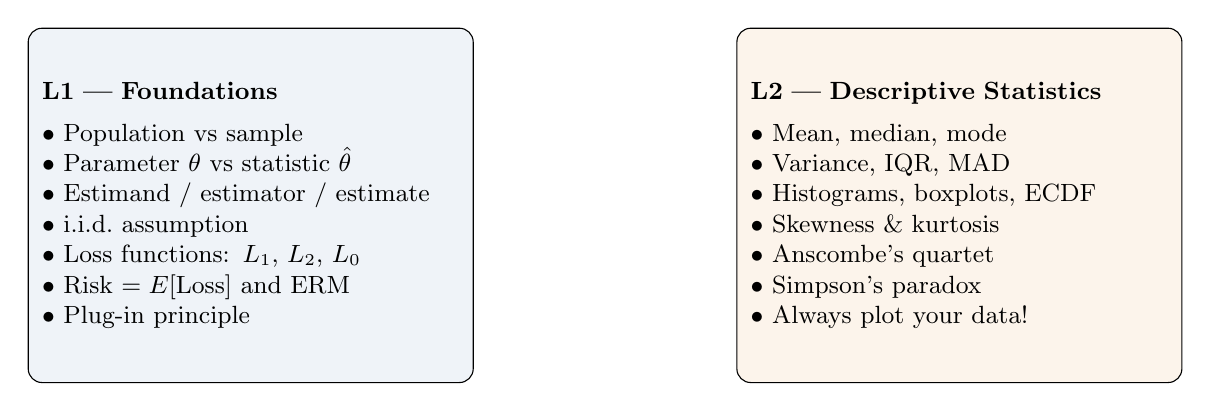
\begin{tikzpicture}[
  cbox/.style={draw, rounded corners=5pt, text width=5.3cm, align=left, inner sep=5pt, font=\small, minimum height=4.5cm}
]
  \node[cbox, fill=popblue!8] at (-4.5, 0) {
    \textbf{L1 --- Foundations}\\[4pt]
    $\bullet$ Population vs sample\\
    $\bullet$ Parameter $\theta$ vs statistic $\hat\theta$\\
    $\bullet$ Estimand / estimator / estimate\\
    $\bullet$ i.i.d.\ assumption\\
    $\bullet$ Loss functions: $L_1$, $L_2$, $L_0$\\
    $\bullet$ Risk $=E[\text{Loss}]$ and ERM\\
    $\bullet$ Plug-in principle
  };
  \node[cbox, fill=orange1!8] at (4.5, 0) {
    \textbf{L2 --- Descriptive Statistics}\\[4pt]
    $\bullet$ Mean, median, mode\\
    $\bullet$ Variance, IQR, MAD\\
    $\bullet$ Histograms, boxplots, ECDF\\
    $\bullet$ Skewness \& kurtosis\\
    $\bullet$ Anscombe's quartet\\
    $\bullet$ Simpson's paradox\\
    $\bullet$ Always plot your data!
  };
\end{tikzpicture}
\end{center}

\vspace{0.1cm}
\begin{center}

\begin{tikzpicture}
  \node[draw=orange1, fill=orange1!5, rounded corners=5pt, text width=10cm, align=center, inner sep=5pt, font=\small] {
    \textbf{Key lesson:} Statistics begins with a question about a \textit{population}, answered using a \textit{sample}.
  };
\end{tikzpicture}
\end{center}
\end{frame}

% ============================================================
% BLOCK 2: ESTIMATOR PROPERTIES
% ============================================================
\begin{frame}
\frametitle{L3--L4: Properties of Estimators}

\begin{center}
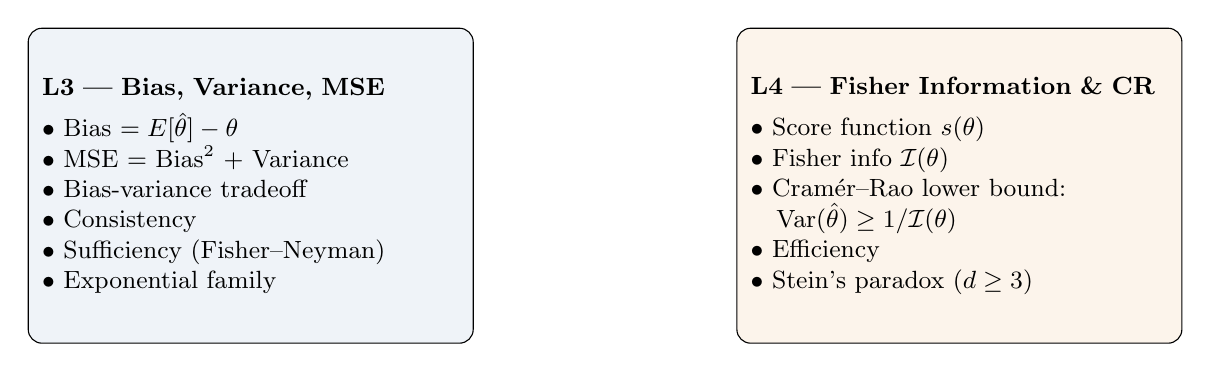
\begin{tikzpicture}[
  cbox/.style={draw, rounded corners=5pt, text width=5.3cm, align=left, inner sep=5pt, font=\small, minimum height=4cm}
]
  \node[cbox, fill=popblue!8] at (-4.5, 0) {
    \textbf{L3 --- Bias, Variance, MSE}\\[4pt]
    $\bullet$ Bias $= E[\hat\theta] - \theta$\\
    $\bullet$ MSE $=$ Bias$^2$ $+$ Variance\\
    $\bullet$ Bias-variance tradeoff\\
    $\bullet$ Consistency\\
    $\bullet$ Sufficiency (Fisher--Neyman)\\
    $\bullet$ Exponential family
  };
  \node[cbox, fill=orange1!8] at (4.5, 0) {
    \textbf{L4 --- Fisher Information \& CR}\\[4pt]
    $\bullet$ Score function $s(\theta)$\\
    $\bullet$ Fisher info $\mathcal{I}(\theta)$\\
    $\bullet$ Cram\'er--Rao lower bound:\\
    \quad $\text{Var}(\hat\theta) \ge 1/\mathcal{I}(\theta)$\\
    $\bullet$ Efficiency\\
    $\bullet$ Stein's paradox ($d \ge 3$)
  };
\end{tikzpicture}
\end{center}

\vspace{0.1cm}
\begin{center}
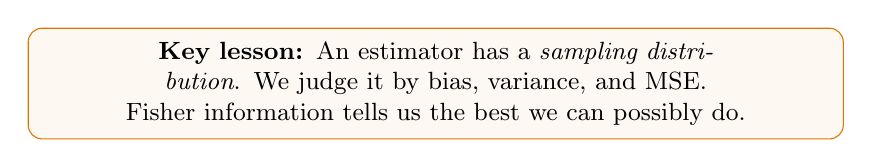
\begin{tikzpicture}
  \node[draw=orange1, fill=orange1!5, rounded corners=5pt, text width=10cm, align=center, inner sep=5pt, font=\small] {
    \textbf{Key lesson:} An estimator has a \textit{sampling distribution}. We judge it by bias, variance, and MSE.\\
    Fisher information tells us the best we can possibly do.
  };
\end{tikzpicture}
\end{center}
\end{frame}

% ============================================================
% BLOCK 3: POINT ESTIMATION
% ============================================================
\begin{frame}
\frametitle{L5--L6: Point Estimation --- MLE \& MAP}

\begin{center}
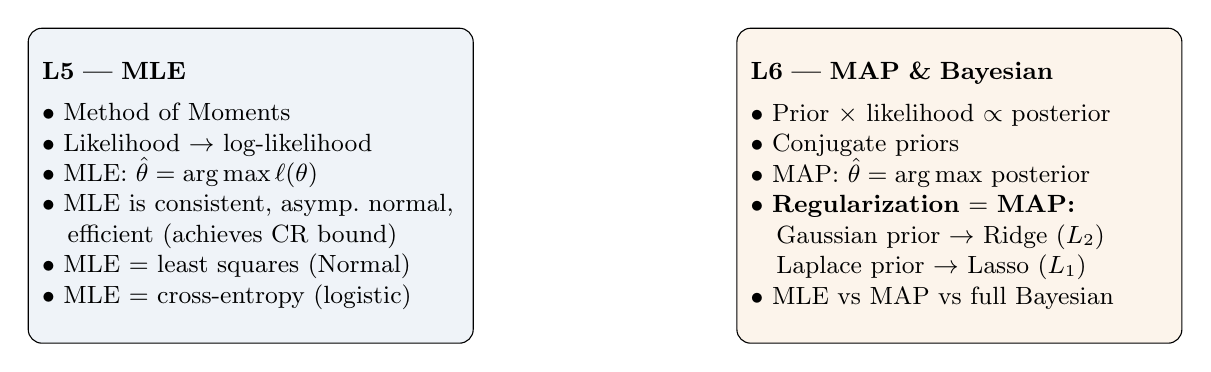
\begin{tikzpicture}[
  cbox/.style={draw, rounded corners=5pt, text width=5.3cm, align=left, inner sep=5pt, font=\small, minimum height=4cm}
]
  \node[cbox, fill=popblue!8] at (-4.5, 0) {
    \textbf{L5 --- MLE}\\[4pt]
    $\bullet$ Method of Moments\\
    $\bullet$ Likelihood $\to$ log-likelihood\\
    $\bullet$ MLE: $\hat\theta = \arg\max \ell(\theta)$\\
    $\bullet$ MLE is consistent, asymp.\ normal,\\
    \quad efficient (achieves CR bound)\\
    $\bullet$ MLE $=$ least squares (Normal)\\
    $\bullet$ MLE $=$ cross-entropy (logistic)
  };
  \node[cbox, fill=orange1!8] at (4.5, 0) {
    \textbf{L6 --- MAP \& Bayesian}\\[4pt]
    $\bullet$ Prior $\times$ likelihood $\propto$ posterior\\
    $\bullet$ Conjugate priors\\
    $\bullet$ MAP: $\hat\theta = \arg\max$ posterior\\
    $\bullet$ \textbf{Regularization $=$ MAP:}\\
    \quad Gaussian prior $\to$ Ridge ($L_2$)\\
    \quad Laplace prior $\to$ Lasso ($L_1$)\\
    $\bullet$ MLE vs MAP vs full Bayesian
  };
\end{tikzpicture}
\end{center}

\vspace{0.1cm}
\begin{center}
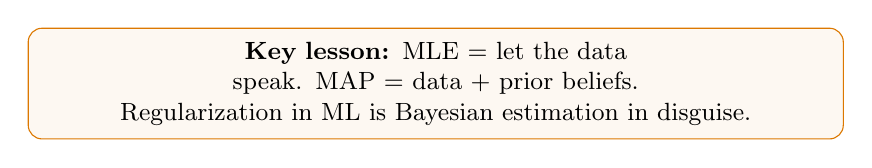
\begin{tikzpicture}
  \node[draw=orange1, fill=orange1!5, rounded corners=5pt, text width=10cm, align=center, inner sep=5pt, font=\small] {
    \textbf{Key lesson:} MLE = let the data speak. MAP = data + prior beliefs.\\
    Regularization in ML is Bayesian estimation in disguise.
  };
\end{tikzpicture}
\end{center}
\end{frame}

% ============================================================
% BLOCK 4: SAMPLING DISTRIBUTIONS & CIs
% ============================================================
\begin{frame}
\frametitle{L7--L8: Sampling Distributions, CIs \& Bootstrap}

\begin{center}
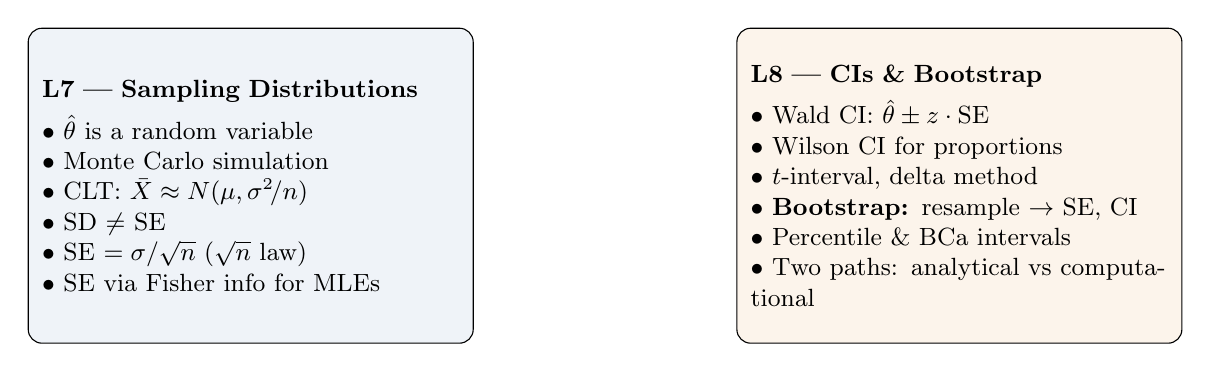
\begin{tikzpicture}[
  cbox/.style={draw, rounded corners=5pt, text width=5.3cm, align=left, inner sep=5pt, font=\small, minimum height=4cm}
]
  \node[cbox, fill=popblue!8] at (-4.5, 0) {
    \textbf{L7 --- Sampling Distributions}\\[4pt]
    $\bullet$ $\hat\theta$ is a random variable\\
    $\bullet$ Monte Carlo simulation\\
    $\bullet$ CLT: $\bar X \approx N(\mu, \sigma^2\!/n)$\\
    $\bullet$ SD $\neq$ SE\\
    $\bullet$ SE $= \sigma/\sqrt{n}$ ($\sqrt{n}$ law)\\
    $\bullet$ SE via Fisher info for MLEs
  };
  \node[cbox, fill=orange1!8] at (4.5, 0) {
    \textbf{L8 --- CIs \& Bootstrap}\\[4pt]
    $\bullet$ Wald CI: $\hat\theta \pm z \cdot \text{SE}$\\
    $\bullet$ Wilson CI for proportions\\
    $\bullet$ $t$-interval, delta method\\
    $\bullet$ \textbf{Bootstrap:} resample $\to$ SE, CI\\
    $\bullet$ Percentile \& BCa intervals\\
    $\bullet$ Two paths: analytical vs computational
  };
\end{tikzpicture}
\end{center}

\vspace{0.1cm}
\begin{center}
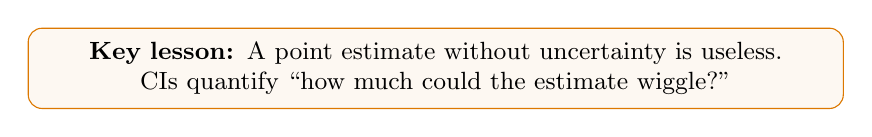
\begin{tikzpicture}
  \node[draw=orange1, fill=orange1!5, rounded corners=5pt, text width=10cm, align=center, inner sep=5pt, font=\small] {
    \textbf{Key lesson:} A point estimate without uncertainty is useless.\\
    CIs quantify ``how much could the estimate wiggle?''
  };
\end{tikzpicture}
\end{center}
\end{frame}

% ============================================================
% BLOCK 5: HYPOTHESIS TESTING
% ============================================================
\begin{frame}
\frametitle{L9--L10: Hypothesis Testing \& Classical Tests}

\begin{center}
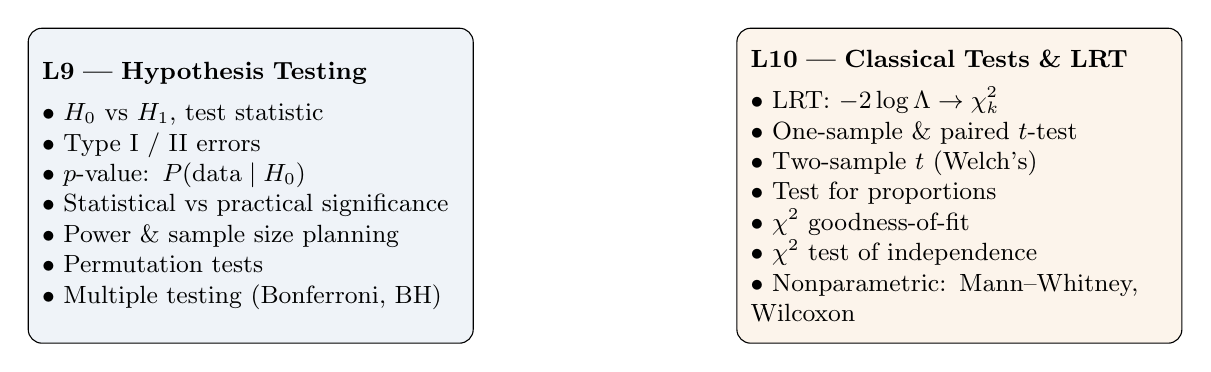
\begin{tikzpicture}[
  cbox/.style={draw, rounded corners=5pt, text width=5.3cm, align=left, inner sep=5pt, font=\small, minimum height=4cm}
]
  \node[cbox, fill=popblue!8] at (-4.5, 0) {
    \textbf{L9 --- Hypothesis Testing}\\[4pt]
    $\bullet$ $H_0$ vs $H_1$, test statistic\\
    $\bullet$ Type I / II errors\\
    $\bullet$ $p$-value: $P(\text{data} \mid H_0)$\\
    $\bullet$ Statistical vs practical significance\\
    $\bullet$ Power \& sample size planning\\
    $\bullet$ Permutation tests\\
    $\bullet$ Multiple testing (Bonferroni, BH)
  };
  \node[cbox, fill=orange1!8] at (4.5, 0) {
    \textbf{L10 --- Classical Tests \& LRT}\\[4pt]
    $\bullet$ LRT: $-2\log\Lambda \to \chi^2_k$\\
    $\bullet$ One-sample \& paired $t$-test\\
    $\bullet$ Two-sample $t$ (Welch's)\\
    $\bullet$ Test for proportions\\
    $\bullet$ $\chi^2$ goodness-of-fit\\
    $\bullet$ $\chi^2$ test of independence\\
    $\bullet$ Nonparametric: Mann--Whitney, Wilcoxon
  };
\end{tikzpicture}
\end{center}

\vspace{0.1cm}
\begin{center}

\begin{tikzpicture}
  \node[draw=orange1, fill=orange1!5, rounded corners=5pt, text width=10cm, align=center, inner sep=5pt, font=\small] {
    \textbf{Key lesson:} A $p$-value asks ``how surprising is the data if $H_0$ is true?''\\
    Small $p$ $\neq$ large effect. Always report effect sizes.
  };
\end{tikzpicture}
\end{center}
\end{frame}

% ============================================================
% BLOCK 6: ANOVA & A/B
% ============================================================
\begin{frame}
\frametitle{L11: ANOVA \& A/B Testing}

\begin{center}
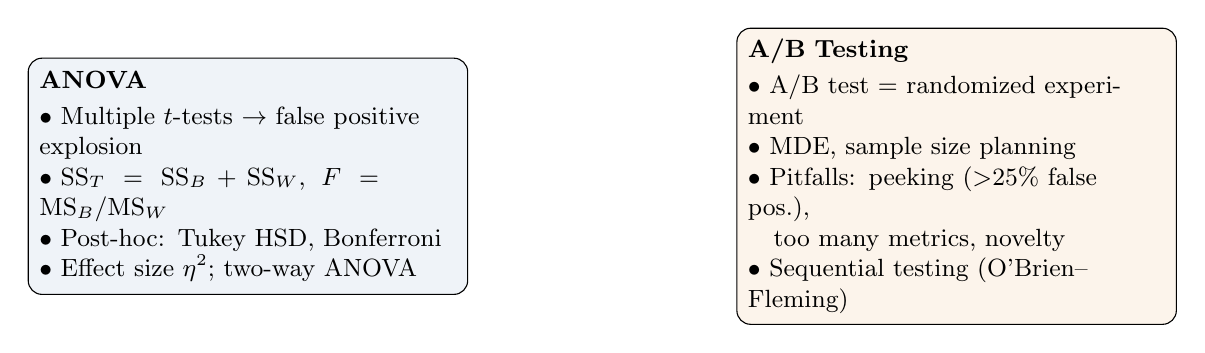
\begin{tikzpicture}[
  cbox/.style={draw, rounded corners=5pt, text width=5.3cm, align=left, inner sep=4pt, font=\small, minimum height=3cm}
]
  \node[cbox, fill=popblue!8] at (-4.5, 0) {
    \textbf{ANOVA}\\[2pt]
    $\bullet$ Multiple $t$-tests $\to$ false positive explosion\\
    $\bullet$ $\text{SS}_T = \text{SS}_B + \text{SS}_W$, \;$F = \text{MS}_B / \text{MS}_W$\\
    $\bullet$ Post-hoc: Tukey HSD, Bonferroni\\
    $\bullet$ Effect size $\eta^2$; two-way ANOVA
  };
  \node[cbox, fill=orange1!8] at (4.5, 0) {
    \textbf{A/B Testing}\\[2pt]
    $\bullet$ A/B test $=$ randomized experiment\\
    $\bullet$ MDE, sample size planning\\
    $\bullet$ Pitfalls: peeking ($>$25\% false pos.),\\
    \quad too many metrics, novelty\\
    $\bullet$ Sequential testing (O'Brien--Fleming)
  };
\end{tikzpicture}
\end{center}

\vspace{0.05cm}
\begin{center}
\small\textbf{Key lesson:} Comparing $k$ groups needs ANOVA, not $\binom{k}{2}$ $t$-tests. A/B testing = hypothesis testing for products.
\end{center}
\end{frame}

% ============================================================
% BLOCK 7: REGRESSION & GLMs
% ============================================================
\begin{frame}
\frametitle{L12--L13: Regression Inference \& GLMs}

\begin{center}
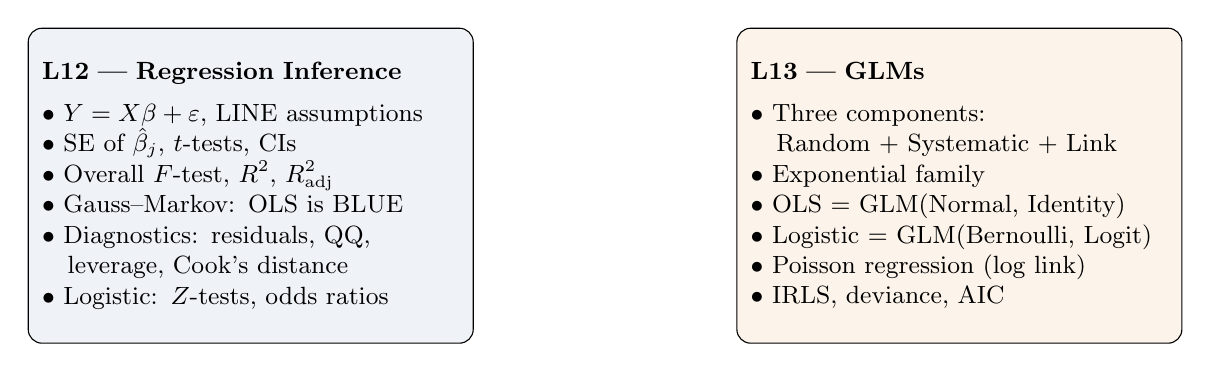
\begin{tikzpicture}[
  cbox/.style={draw, rounded corners=5pt, text width=5.3cm, align=left, inner sep=5pt, font=\small, minimum height=4cm}
]
  \node[cbox, fill=popblue!8] at (-4.5, 0) {
    \textbf{L12 --- Regression Inference}\\[4pt]
    $\bullet$ $Y = X\beta + \varepsilon$, LINE assumptions\\
    $\bullet$ SE of $\hat\beta_j$, $t$-tests, CIs\\
    $\bullet$ Overall $F$-test, $R^2$, $R^2_\text{adj}$\\
    $\bullet$ Gauss--Markov: OLS is BLUE\\
    $\bullet$ Diagnostics: residuals, QQ,\\
    \quad leverage, Cook's distance\\
    $\bullet$ Logistic: $Z$-tests, odds ratios
  };
  \node[cbox, fill=orange1!8] at (4.5, 0) {
    \textbf{L13 --- GLMs}\\[4pt]
    $\bullet$ Three components:\\
    \quad Random + Systematic + Link\\
    $\bullet$ Exponential family\\
    $\bullet$ OLS $=$ GLM(Normal, Identity)\\
    $\bullet$ Logistic $=$ GLM(Bernoulli, Logit)\\
    $\bullet$ Poisson regression (log link)\\
    $\bullet$ IRLS, deviance, AIC
  };
\end{tikzpicture}
\end{center}

\vspace{0.1cm}
\begin{center}
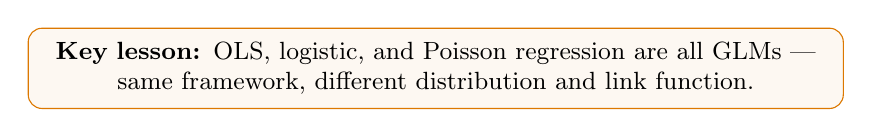
\begin{tikzpicture}
  \node[draw=orange1, fill=orange1!5, rounded corners=5pt, text width=10cm, align=center, inner sep=5pt, font=\small] {
    \textbf{Key lesson:} OLS, logistic, and Poisson regression are all GLMs ---\\
    same framework, different distribution and link function.
  };
\end{tikzpicture}
\end{center}
\end{frame}

% ============================================================
% BLOCK 8: CAUSAL INFERENCE
% ============================================================
\begin{frame}
\frametitle{L14: Causal Inference}

\begin{center}
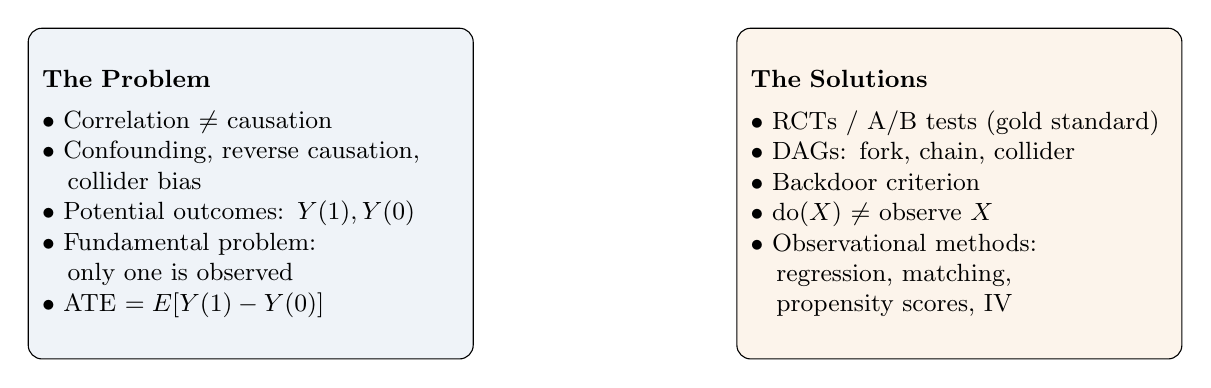
\begin{tikzpicture}[
  cbox/.style={draw, rounded corners=5pt, text width=5.3cm, align=left, inner sep=5pt, font=\small, minimum height=4.2cm}
]
  \node[cbox, fill=popblue!8] at (-4.5, 0) {
    \textbf{The Problem}\\[4pt]
    $\bullet$ Correlation $\neq$ causation\\
    $\bullet$ Confounding, reverse causation,\\
    \quad collider bias\\
    $\bullet$ Potential outcomes: $Y(1), Y(0)$\\
    $\bullet$ Fundamental problem:\\
    \quad only one is observed\\
    $\bullet$ ATE $= E[Y(1) - Y(0)]$
  };
  \node[cbox, fill=orange1!8] at (4.5, 0) {
    \textbf{The Solutions}\\[4pt]
    $\bullet$ RCTs / A/B tests (gold standard)\\
    $\bullet$ DAGs: fork, chain, collider\\
    $\bullet$ Backdoor criterion\\
    $\bullet$ do($X$) $\neq$ observe $X$\\
    $\bullet$ Observational methods:\\
    \quad regression, matching,\\
    \quad propensity scores, IV
  };
\end{tikzpicture}
\end{center}

\vspace{0.1cm}
\begin{center}
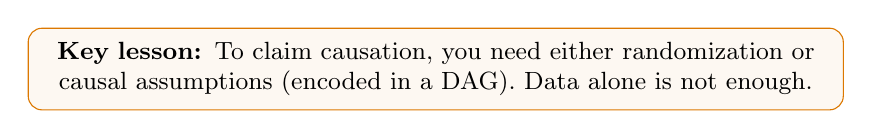
\begin{tikzpicture}
  \node[draw=orange1, fill=orange1!5, rounded corners=5pt, text width=10cm, align=center, inner sep=5pt, font=\small] {
    \textbf{Key lesson:} To claim causation, you need either randomization or\\
    causal assumptions (encoded in a DAG). Data alone is not enough.
  };
\end{tikzpicture}
\end{center}
\end{frame}

% ============================================================
% THE BIG FORMULAS
% ============================================================
\begin{frame}
\frametitle{The Formulas That Matter Most}

\begin{center}
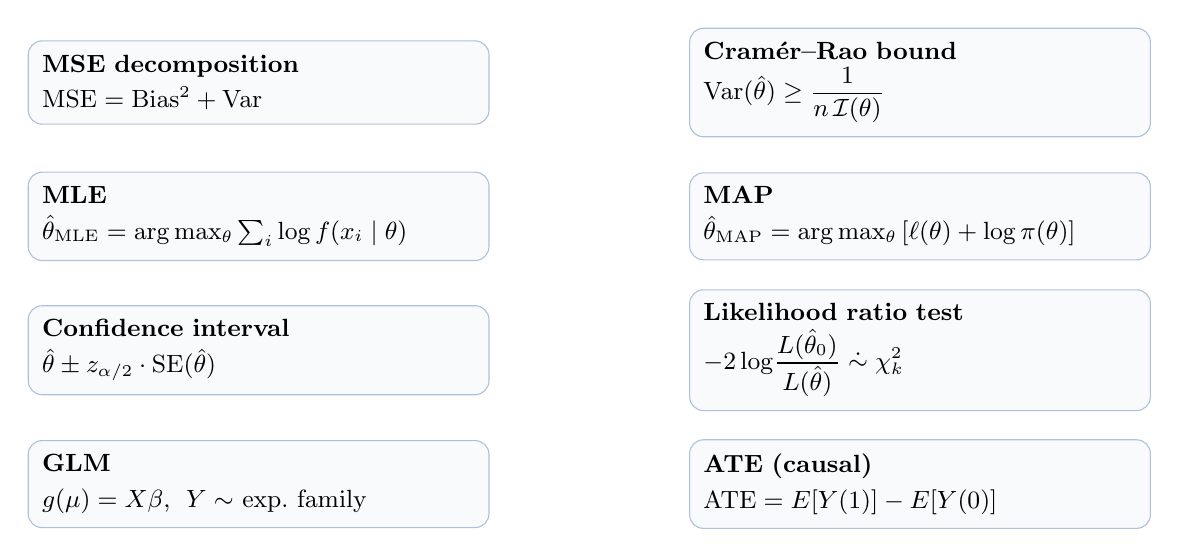
\begin{tikzpicture}[
  fbox/.style={draw=popblue!40, fill=popblue!3, rounded corners=5pt, text width=5.5cm, align=left, inner sep=5pt, font=\small}
]
  \node[fbox] at (-4.2, 2.5) {
    \textbf{MSE decomposition}\\[2pt]
    $\text{MSE} = \text{Bias}^2 + \text{Var}$
  };
  \node[fbox] at (4.2, 2.5) {
    \textbf{Cram\'er--Rao bound}\\[2pt]
    $\text{Var}(\hat\theta) \ge \dfrac{1}{n\,\mathcal{I}(\theta)}$
  };
  \node[fbox] at (-4.2, 0.8) {
    \textbf{MLE}\\[2pt]
    $\hat\theta_\text{MLE} = \arg\max_\theta \sum_i \log f(x_i \mid \theta)$
  };
  \node[fbox] at (4.2, 0.8) {
    \textbf{MAP}\\[2pt]
    $\hat\theta_\text{MAP} = \arg\max_\theta \left[\ell(\theta) + \log\pi(\theta)\right]$
  };
  \node[fbox] at (-4.2, -0.9) {
    \textbf{Confidence interval}\\[2pt]
    $\hat\theta \pm z_{\alpha/2} \cdot \text{SE}(\hat\theta)$
  };
  \node[fbox] at (4.2, -0.9) {
    \textbf{Likelihood ratio test}\\[2pt]
    $-2\log\!\dfrac{L(\hat\theta_0)}{L(\hat\theta)} \;\dot\sim\; \chi^2_k$
  };
  \node[fbox] at (-4.2, -2.6) {
    \textbf{GLM}\\[2pt]
    $g(\mu) = X\beta$, \;$Y \sim$ exp.\ family
  };
  \node[fbox] at (4.2, -2.6) {
    \textbf{ATE (causal)}\\[2pt]
    $\text{ATE} = E[Y(1)] - E[Y(0)]$
  };
\end{tikzpicture}
\end{center}
\end{frame}

% ============================================================
% THE RECURRING THEMES
% ============================================================
\begin{frame}
\frametitle{Five Themes That Connect Everything}

\begin{center}
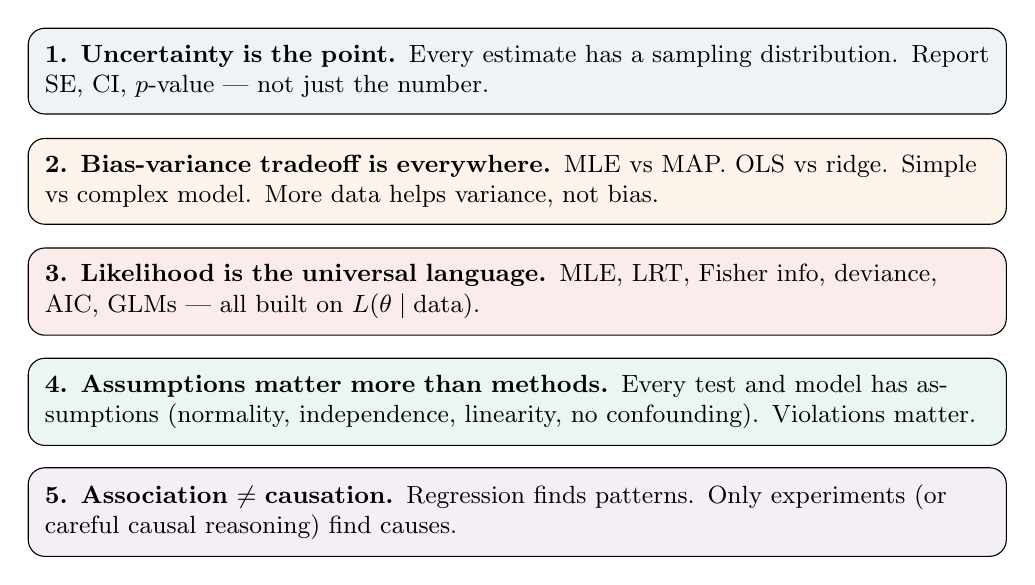
\begin{tikzpicture}[
  tbox/.style={draw, rounded corners=6pt, text width=12cm, align=left, inner sep=6pt, font=\small, minimum height=0.8cm}
]
  \node[tbox, fill=popblue!8] at (0, 3.0) {
    \textbf{1. Uncertainty is the point.}
    Every estimate has a sampling distribution. Report SE, CI, $p$-value --- not just the number.
  };
  \node[tbox, fill=orange1!8] at (0, 1.6) {
    \textbf{2. Bias-variance tradeoff is everywhere.}
    MLE vs MAP. OLS vs ridge. Simple vs complex model. More data helps variance, not bias.
  };
  \node[tbox, fill=sampred!8] at (0, 0.2) {
    \textbf{3. Likelihood is the universal language.}
    MLE, LRT, Fisher info, deviance, AIC, GLMs --- all built on $L(\theta \mid \text{data})$.
  };
  \node[tbox, fill=paramgreen!8] at (0, -1.2) {
    \textbf{4. Assumptions matter more than methods.}
    Every test and model has assumptions (normality, independence, linearity, no confounding). Violations matter.
  };
  \node[tbox, fill=violet1!8] at (0, -2.6) {
    \textbf{5. Association $\neq$ causation.}
    Regression finds patterns. Only experiments (or careful causal reasoning) find causes.
  };
\end{tikzpicture}
\end{center}
\end{frame}

% ============================================================
% DECISION FLOWCHART
% ============================================================
\begin{frame}
\frametitle{Which Method Do I Use?}

\begin{center}
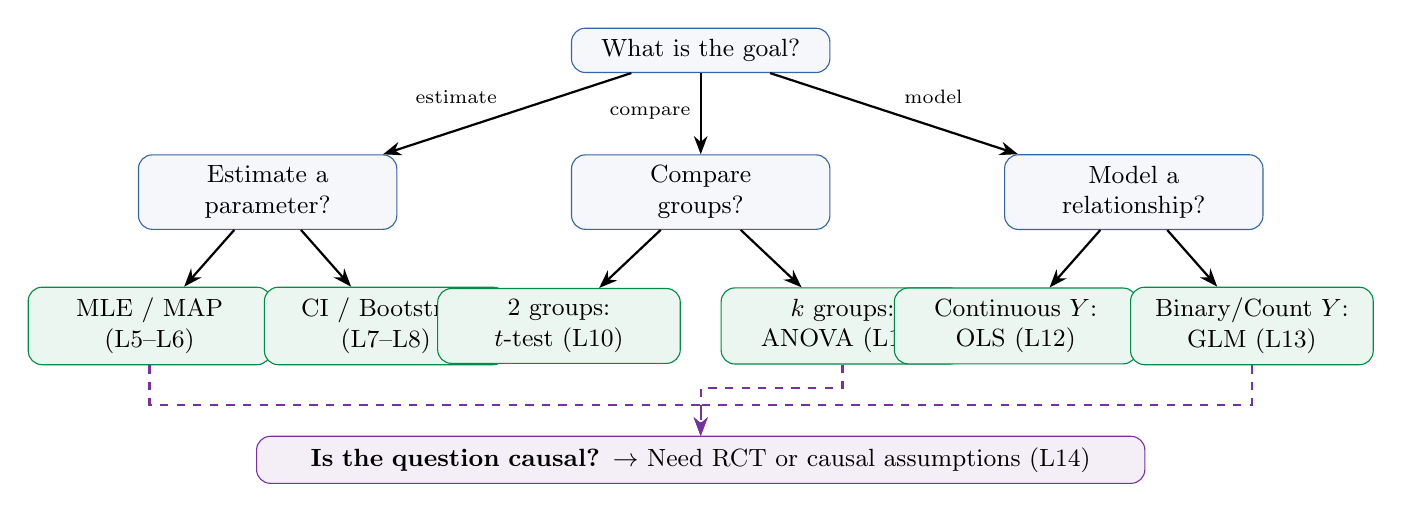
\begin{tikzpicture}[
  node distance=0.8cm,
  dnode/.style={draw=popblue, fill=popblue!5, rounded corners=5pt, text width=3cm, align=center, inner sep=4pt, font=\small},
  lnode/.style={draw=paramgreen, fill=paramgreen!8, rounded corners=5pt, text width=2.8cm, align=center, inner sep=4pt, font=\small},
  arr/.style={-{Stealth}, thick},
  lbl/.style={font=\scriptsize, midway}
]
  \node[dnode] (q) at (0, 3) {What is the goal?};

  \node[dnode] (est) at (-5.5, 1.2) {Estimate a\\parameter?};
  \node[dnode] (comp) at (0, 1.2) {Compare\\groups?};
  \node[dnode] (rel) at (5.5, 1.2) {Model a\\relationship?};

  \draw[arr] (q) -- (est) node[lbl, above left] {estimate};
  \draw[arr] (q) -- (comp) node[lbl, left] {compare};
  \draw[arr] (q) -- (rel) node[lbl, above right] {model};

  % Estimate branch
  \node[lnode] (mle) at (-7, -0.5) {MLE / MAP\\(L5--L6)};
  \node[lnode] (ci) at (-4, -0.5) {CI / Bootstrap\\(L7--L8)};
  \draw[arr] (est) -- (mle);
  \draw[arr] (est) -- (ci);

  % Compare branch
  \node[lnode] (t2) at (-1.8, -0.5) {2 groups:\\$t$-test (L10)};
  \node[lnode] (ak) at (1.8, -0.5) {$k$ groups:\\ANOVA (L11)};
  \draw[arr] (comp) -- (t2);
  \draw[arr] (comp) -- (ak);

  % Model branch
  \node[lnode] (ols) at (4, -0.5) {Continuous $Y$:\\OLS (L12)};
  \node[lnode] (glm) at (7, -0.5) {Binary/Count $Y$:\\GLM (L13)};
  \draw[arr] (rel) -- (ols);
  \draw[arr] (rel) -- (glm);

  % Causal layer
  \node[draw=violet1, fill=violet1!8, rounded corners=5pt, text width=11cm, align=center, inner sep=4pt, font=\small] (caus) at (0, -2.2) {
    \textbf{Is the question causal?} $\to$ Need RCT or causal assumptions (L14)
  };
  \draw[arr, violet1, dashed] (mle.south) -- ++(0, -0.5) -| (caus);
  \draw[arr, violet1, dashed] (ak.south) -- ++(0, -0.3) -| (caus);
  \draw[arr, violet1, dashed] (glm.south) -- ++(0, -0.5) -| (caus);
\end{tikzpicture}
\end{center}
\end{frame}

% ============================================================
% COMMON MISTAKES
% ============================================================
\begin{frame}
\frametitle{Top Mistakes to Avoid}

\begin{center}
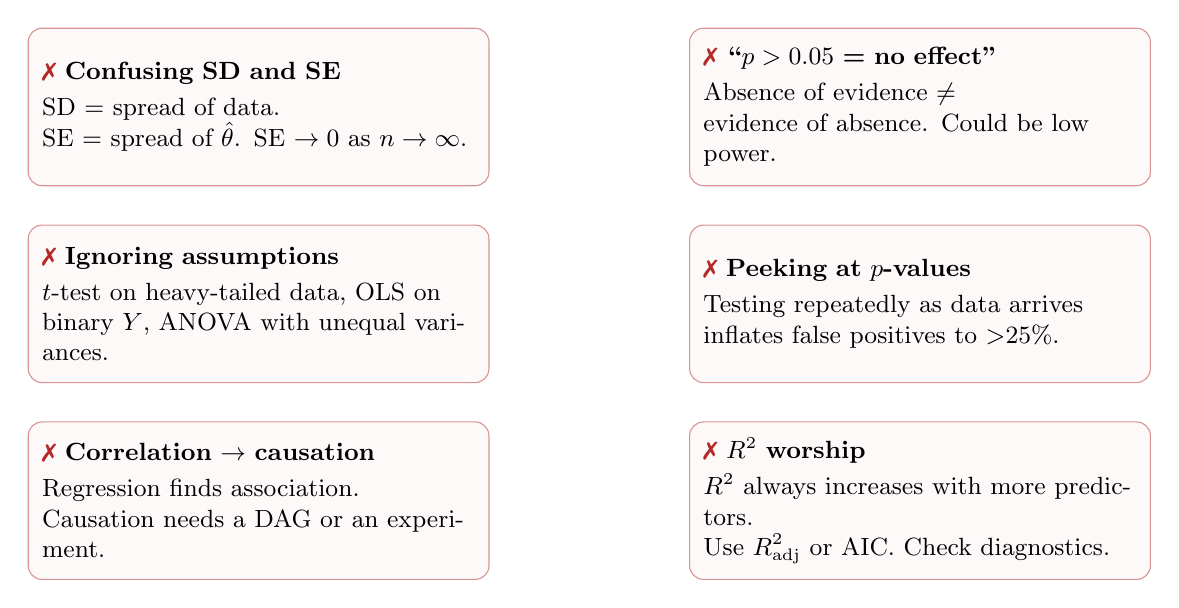
\begin{tikzpicture}[
  mbox/.style={draw=warnred!50, fill=warnred!3, rounded corners=5pt, text width=5.5cm, align=left, inner sep=5pt, font=\small, minimum height=2cm}
]
  \node[mbox] at (-4.2, 2) {
    \textbf{\textcolor{warnred}{\ding{55}} Confusing SD and SE}\\[2pt]
    SD = spread of data.\\
    SE = spread of $\hat\theta$. SE $\to 0$ as $n \to \infty$.
  };
  \node[mbox] at (4.2, 2) {
    \textbf{\textcolor{warnred}{\ding{55}} ``$p > 0.05$ = no effect''}\\[2pt]
    Absence of evidence $\neq$\\evidence of absence. Could be low power.
  };
  \node[mbox] at (-4.2, -0.5) {
    \textbf{\textcolor{warnred}{\ding{55}} Ignoring assumptions}\\[2pt]
    $t$-test on heavy-tailed data, OLS on\\binary $Y$, ANOVA with unequal variances.
  };
  \node[mbox] at (4.2, -0.5) {
    \textbf{\textcolor{warnred}{\ding{55}} Peeking at $p$-values}\\[2pt]
    Testing repeatedly as data arrives\\inflates false positives to $>$25\%.
  };
  \node[mbox] at (-4.2, -3) {
    \textbf{\textcolor{warnred}{\ding{55}} Correlation $\to$ causation}\\[2pt]
    Regression finds association.\\
    Causation needs a DAG or an experiment.
  };
  \node[mbox] at (4.2, -3) {
    \textbf{\textcolor{warnred}{\ding{55}} $R^2$ worship}\\[2pt]
    $R^2$ always increases with more predictors.\\
    Use $R^2_\text{adj}$ or AIC. Check diagnostics.
  };
\end{tikzpicture}
\end{center}
\end{frame}

% ============================================================
% PYTHON TOOLKIT
% ============================================================
\begin{frame}
\frametitle{Your Python Toolkit}

\begin{center}
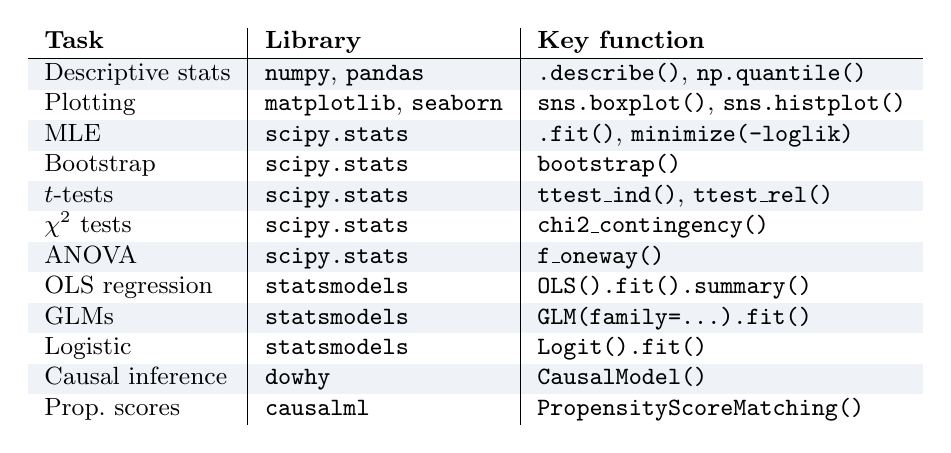
\begin{tikzpicture}
  \node[inner sep=0pt] {
    \small
    \begin{tabular}{l|l|l}
      \textbf{Task} & \textbf{Library} & \textbf{Key function} \\
      \hline
      \rowcolor{popblue!8}
      Descriptive stats & \texttt{numpy}, \texttt{pandas} & \texttt{.describe()}, \texttt{np.quantile()} \\
      Plotting & \texttt{matplotlib}, \texttt{seaborn} & \texttt{sns.boxplot()}, \texttt{sns.histplot()} \\
      \rowcolor{popblue!8}
      MLE & \texttt{scipy.stats} & \texttt{.fit()}, \texttt{minimize(-loglik)} \\
      Bootstrap & \texttt{scipy.stats} & \texttt{bootstrap()} \\
      \rowcolor{popblue!8}
      $t$-tests & \texttt{scipy.stats} & \texttt{ttest\_ind()}, \texttt{ttest\_rel()} \\
      $\chi^2$ tests & \texttt{scipy.stats} & \texttt{chi2\_contingency()} \\
      \rowcolor{popblue!8}
      ANOVA & \texttt{scipy.stats} & \texttt{f\_oneway()} \\
      OLS regression & \texttt{statsmodels} & \texttt{OLS().fit().summary()} \\
      \rowcolor{popblue!8}
      GLMs & \texttt{statsmodels} & \texttt{GLM(family=...).fit()} \\
      Logistic & \texttt{statsmodels} & \texttt{Logit().fit()} \\
      \rowcolor{popblue!8}
      Causal inference & \texttt{dowhy} & \texttt{CausalModel()} \\
      Prop.\ scores & \texttt{causalml} & \texttt{PropensityScoreMatching()} \\
    \end{tabular}
  };
\end{tikzpicture}
\end{center}
\end{frame}

% ============================================================
% WHAT TO LEARN NEXT
% ============================================================
\begin{frame}
\frametitle{Where to Go Next}

\begin{center}
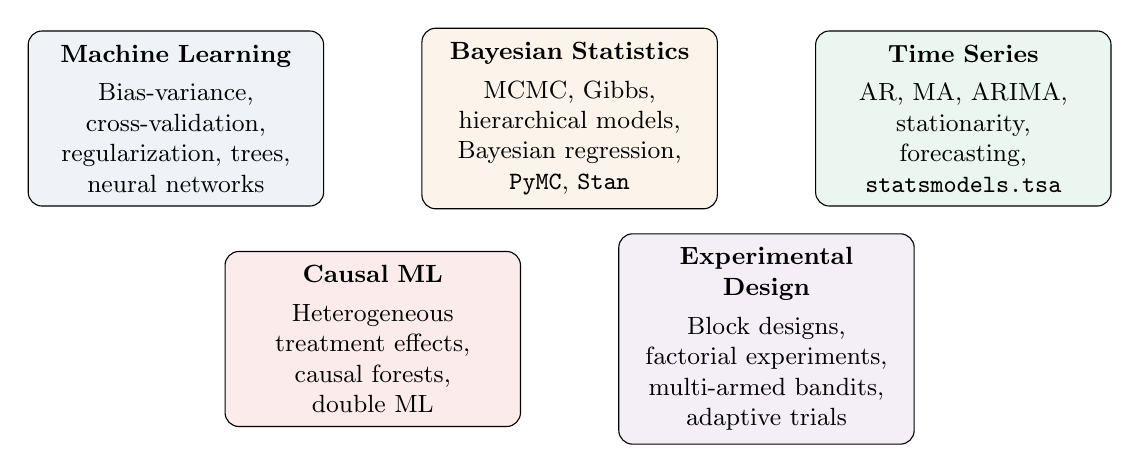
\begin{tikzpicture}[
  nbox/.style={draw, rounded corners=5pt, text width=3.4cm, align=center, inner sep=5pt, font=\small, minimum height=2.2cm}
]
  \node[nbox, fill=popblue!8] at (-5, 1.5) {
    \textbf{Machine Learning}\\[3pt]
    Bias-variance,\\
    cross-validation,\\
    regularization, trees,\\
    neural networks
  };
  \node[nbox, fill=orange1!8] at (0, 1.5) {
    \textbf{Bayesian Statistics}\\[3pt]
    MCMC, Gibbs,\\
    hierarchical models,\\
    Bayesian regression,\\
    \texttt{PyMC}, \texttt{Stan}
  };
  \node[nbox, fill=paramgreen!8] at (5, 1.5) {
    \textbf{Time Series}\\[3pt]
    AR, MA, ARIMA,\\
    stationarity,\\
    forecasting,\\
    \texttt{statsmodels.tsa}
  };
  \node[nbox, fill=sampred!8] at (-2.5, -1.3) {
    \textbf{Causal ML}\\[3pt]
    Heterogeneous\\
    treatment effects,\\
    causal forests,\\
    double ML
  };
  \node[nbox, fill=violet1!8] at (2.5, -1.3) {
    \textbf{Experimental Design}\\[3pt]
    Block designs,\\
    factorial experiments,\\
    multi-armed bandits,\\
    adaptive trials
  };
\end{tikzpicture}
\end{center}
\end{frame}

% ============================================================
% CLOSING
% ============================================================
\begin{frame}
\begin{center}
  \vspace{1.5cm}
  {\Huge\bfseries\textcolor{popblue}{That's Statistics!}}

  \vspace{0.8cm}
  {\large 14 lectures $\cdot$ From data to causation}

  \vspace{0.8cm}
  
\begin{tikzpicture}
    \node[draw=popblue, fill=popblue!5, rounded corners=8pt, text width=10cm, align=center, inner sep=8pt, font=\small] {
      \textit{``All models are wrong, but some are useful.''}\\[4pt]
      --- George E.\ P.\ Box
    };
  \end{tikzpicture}
\end{center}
\end{frame}

\end{document}
